\documentclass[twocolumn,10pt]{article}
\usepackage[margin=1.8cm]{geometry}
\usepackage{amsmath,amssymb,amsthm}
\usepackage{graphicx}
\usepackage{booktabs}
\usepackage{hyperref}
\usepackage{xcolor}
\usepackage{algorithm}
\usepackage{algpseudocode}
\usepackage{bbm}
\usepackage{physics}
\usepackage{microtype}
\usepackage{subcaption}
\usepackage[numbers,sort&compress]{natbib}

\definecolor{qtclblue}{RGB}{33,150,243}
\definecolor{darkgray}{RGB}{40,40,40}

\title{\textbf{Quantum Transfer Continual Learning}\\
\large Mitigating Catastrophic Forgetting in Variational Quantum Classifiers\\
via Parameter Transfer, Elastic Weight Consolidation, and Quantum Rehearsal}

\author{
  Daniel Martínez Pérez\\
  \small Quantum Machine Learning Group\\
  \small Universidad Pablo de Olavide, Sevilla, Spain\\
  \small \texttt{dmarper2@upo.es}
}
\date{March 2026}

\begin{document}
\maketitle

\begin{abstract}
Continual learning---the ability of a model to acquire new knowledge without
forgetting previously learned tasks---remains one of the central open problems
in machine learning.
Quantum machine learning (QML) introduces an additional challenge: variational
quantum circuits (VQCs) are trained on classical optimizers over highly
non-convex loss landscapes, making them especially susceptible to catastrophic
forgetting when tasks are presented sequentially.
We propose \textbf{Quantum Transfer Continual Learning (QTCL)}, a framework
that combines (i)~\emph{quantum parameter transfer} from previous tasks,
(ii)~\emph{Quantum Elastic Weight Consolidation (QEWC)} based on a diagonal
Fisher-information approximation, and (iii)~\emph{quantum rehearsal}---a
lightweight episodic memory retaining 20\% of each past task's training data.
We evaluate QTCL on four sequential binary-classification tasks encoded via
the ZZFeatureMap~\cite{havlicek2019} with a TwoLocal ansatz on 4~qubits,
simulated with Qiskit Aer.
QTCL achieves an Average Accuracy (AA)~of~0.592, the highest among all
quantum baselines, a positive Backward Transfer (BWT~$=+0.011$) indicating
no net forgetting, and a Forgetting score of~0.033---a $57\%$ reduction
compared to naive fine-tuning.
We include full experimental results, 6 diagnostic figures, and open-source
code.
\end{abstract}

\section{Introduction}

Biological intelligence is inherently continual: humans learn new skills
throughout their lives without erasing prior knowledge.
Replicating this ability in artificial systems---\emph{continual learning}
(CL)---is complicated by \emph{catastrophic forgetting}~\cite{mccloskey1989},
the sharp performance degradation on old tasks after learning new ones.

The emergence of quantum machine learning~\cite{biamonte2017,schuld2019}
opens new research directions but also inherits classical challenges.
Variational Quantum Classifiers (VQC) encode data via quantum feature maps
and optimize a parametrized ansatz with hybrid quantum-classical loops.
Their optimization landscape is non-convex, and gradient-based updates on
sequential tasks can destroy previously learned parameter configurations.

\textbf{Contributions.}
\begin{enumerate}
  \item We formalize the \emph{quantum continual learning} setting and
        define standard CL metrics (AA, BWT, FWT, Forgetting) for VQCs.
  \item We propose QTCL, combining parameter transfer, QEWC, and a
        quantum rehearsal buffer.
  \item We provide the first systematic empirical comparison of quantum
        CL strategies with 4 tasks, 4 qubits, and 5 competing methods.
  \item We release all code and data to enable reproducibility.
\end{enumerate}

\section{Background}

\subsection{Variational Quantum Classifiers}

A VQC is composed of a feature map $U_\phi(\mathbf{x})$ that encodes
input $\mathbf{x}\in\mathbb{R}^n$ into a quantum state, followed by a
trainable ansatz $V(\boldsymbol{\theta})$:
\begin{equation}
  \ket{\psi(\mathbf{x},\boldsymbol{\theta})} =
  V(\boldsymbol{\theta})\,U_\phi(\mathbf{x})\ket{0}^{\otimes n}.
\end{equation}
The output is obtained by measuring an observable $M$:
\begin{equation}
  f(\mathbf{x};\boldsymbol{\theta}) =
  \bra{\psi} M \ket{\psi}.
\end{equation}
Parameters $\boldsymbol{\theta}$ are optimized classically to minimize a
cross-entropy loss over a labeled training set.

\subsection{Continual Learning Metrics}

Let $a_{i,j}$ denote the accuracy on task $j$ after training sequentially on
tasks $1,\ldots,i$.
Following~\cite{lopez2017gradient}, we define:
\begin{align}
  \mathrm{AA}  &= \frac{1}{T}\sum_{j=1}^{T} a_{T,j}, \\
  \mathrm{BWT} &= \frac{1}{T-1}\sum_{j=1}^{T-1}(a_{T,j}-a_{j,j}), \\
  \mathrm{FWT} &= \frac{1}{T-1}\sum_{j=2}^{T}(a_{j-1,j}-b_j), \\
  \mathrm{F}   &= \frac{1}{T-1}\sum_{j=1}^{T-1}
                  \bigl(\max_{l\leq T} a_{l,j} - a_{T,j}\bigr),
\end{align}
where $b_j=0.5$ is the random-chance baseline for binary classification and
$T$ is the total number of tasks.

\section{Quantum Transfer Continual Learning}

\subsection{Problem Setting}

Given a sequence of binary classification tasks
$\mathcal{T}_1, \mathcal{T}_2, \ldots, \mathcal{T}_T$, at step $i$ the
learner has access only to data from $\mathcal{T}_i$ (plus a bounded
rehearsal buffer) and must perform well on all tasks $1,\ldots,i$.

\subsection{QTCL Algorithm}

QTCL (Algorithm~\ref{alg:qtcl}) operates in three stages at each task $i$:

\paragraph{(1) Parameter Transfer.}
Initialize the VQC at step $i$ from the optimal parameters
$\boldsymbol{\theta}^{(i-1)}$ of the previous task, perturbed by
small Gaussian noise:
\begin{equation}
  \boldsymbol{\theta}^{(i)}_0 =
  \boldsymbol{\theta}^{(i-1)} + \eta\,\boldsymbol{\epsilon},\quad
  \boldsymbol{\epsilon}\sim\mathcal{N}(\mathbf{0},\mathbf{I}).
\end{equation}
This exploits positive transfer when tasks share structure while allowing
escape from local minima detrimental to task $i$.

\paragraph{(2) Quantum EWC.}
We approximate the Fisher information matrix diagonally:
\begin{equation}
  F_k \approx \mathbb{E}_{\mathbf{x}\sim\mathcal{T}_{i-1}}
  \left[\left(\frac{\partial \log p(\mathbf{x};\boldsymbol{\theta})}
  {\partial \theta_k}\right)^2\right].
\end{equation}
The training objective at task $i$ includes a quadratic penalty:
\begin{equation}
  \mathcal{L}_{\mathrm{QEWC}} = \mathcal{L}_i(\boldsymbol{\theta}) +
  \frac{\lambda}{2}\sum_k F_k
  \bigl(\theta_k - \theta^{(i-1)}_k\bigr)^2.
\end{equation}
Parameters with high Fisher importance are penalized more strongly,
preserving knowledge of past tasks.

\paragraph{(3) Quantum Rehearsal.}
A buffer $\mathcal{B}$ stores a random 20\% sample from each past task.
At step $i$, the model is trained on
$\mathcal{D}_i \cup \mathcal{B}_{1:i-1}$, providing direct supervision
from previous distributions.

\begin{algorithm}[t]
\caption{QTCL: Quantum Transfer Continual Learning}
\label{alg:qtcl}
\begin{algorithmic}[1]
\Require Tasks $\mathcal{T}_1,\ldots,\mathcal{T}_T$; buffer ratio $\rho$;
         noise scale $\eta$; QEWC weight $\lambda$
\State $\boldsymbol{\theta} \leftarrow \text{random}$;
       $\mathcal{B} \leftarrow \emptyset$
\For{$i = 1$ to $T$}
  \State Sample $\mathcal{D}_i$ from $\mathcal{T}_i$
  \State $\mathcal{D}'_i \leftarrow \mathcal{D}_i \cup \mathcal{B}$
  \If{$i > 1$}
    \State $\boldsymbol{\theta}_0 \leftarrow
           \boldsymbol{\theta} + \eta\,\mathcal{N}(\mathbf{0},\mathbf{I})$
    \State Estimate $\{F_k\}$ on $\mathcal{D}_{i-1}$
  \Else
    \State $\boldsymbol{\theta}_0 \leftarrow \text{random}$
  \EndIf
  \State $\boldsymbol{\theta} \leftarrow
         \arg\min_{\boldsymbol{\theta}}
         \mathcal{L}_{\mathrm{QEWC}}(\boldsymbol{\theta};\mathcal{D}'_i)$
         \textbf{initialized at} $\boldsymbol{\theta}_0$
  \State $\mathcal{B} \leftarrow \mathcal{B} \cup
         \text{RandomSample}(\mathcal{D}_i, \rho|\mathcal{D}_i|)$
\EndFor
\end{algorithmic}
\end{algorithm}

\subsection{Circuit Architecture}

We use the ZZFeatureMap~\cite{havlicek2019} with $r_f=1$ repetitions as the
data-encoding layer, followed by a TwoLocal ansatz with $\{R_Y, R_Z\}$
rotations and CNOT entanglement in a linear topology with $r_a=2$
repetitions (Figure~\ref{fig:circuit}).
The total number of trainable parameters is $2\cdot n\cdot r_a + n = 36$
for $n=4$ qubits.

\begin{figure}[t]
  \centering
  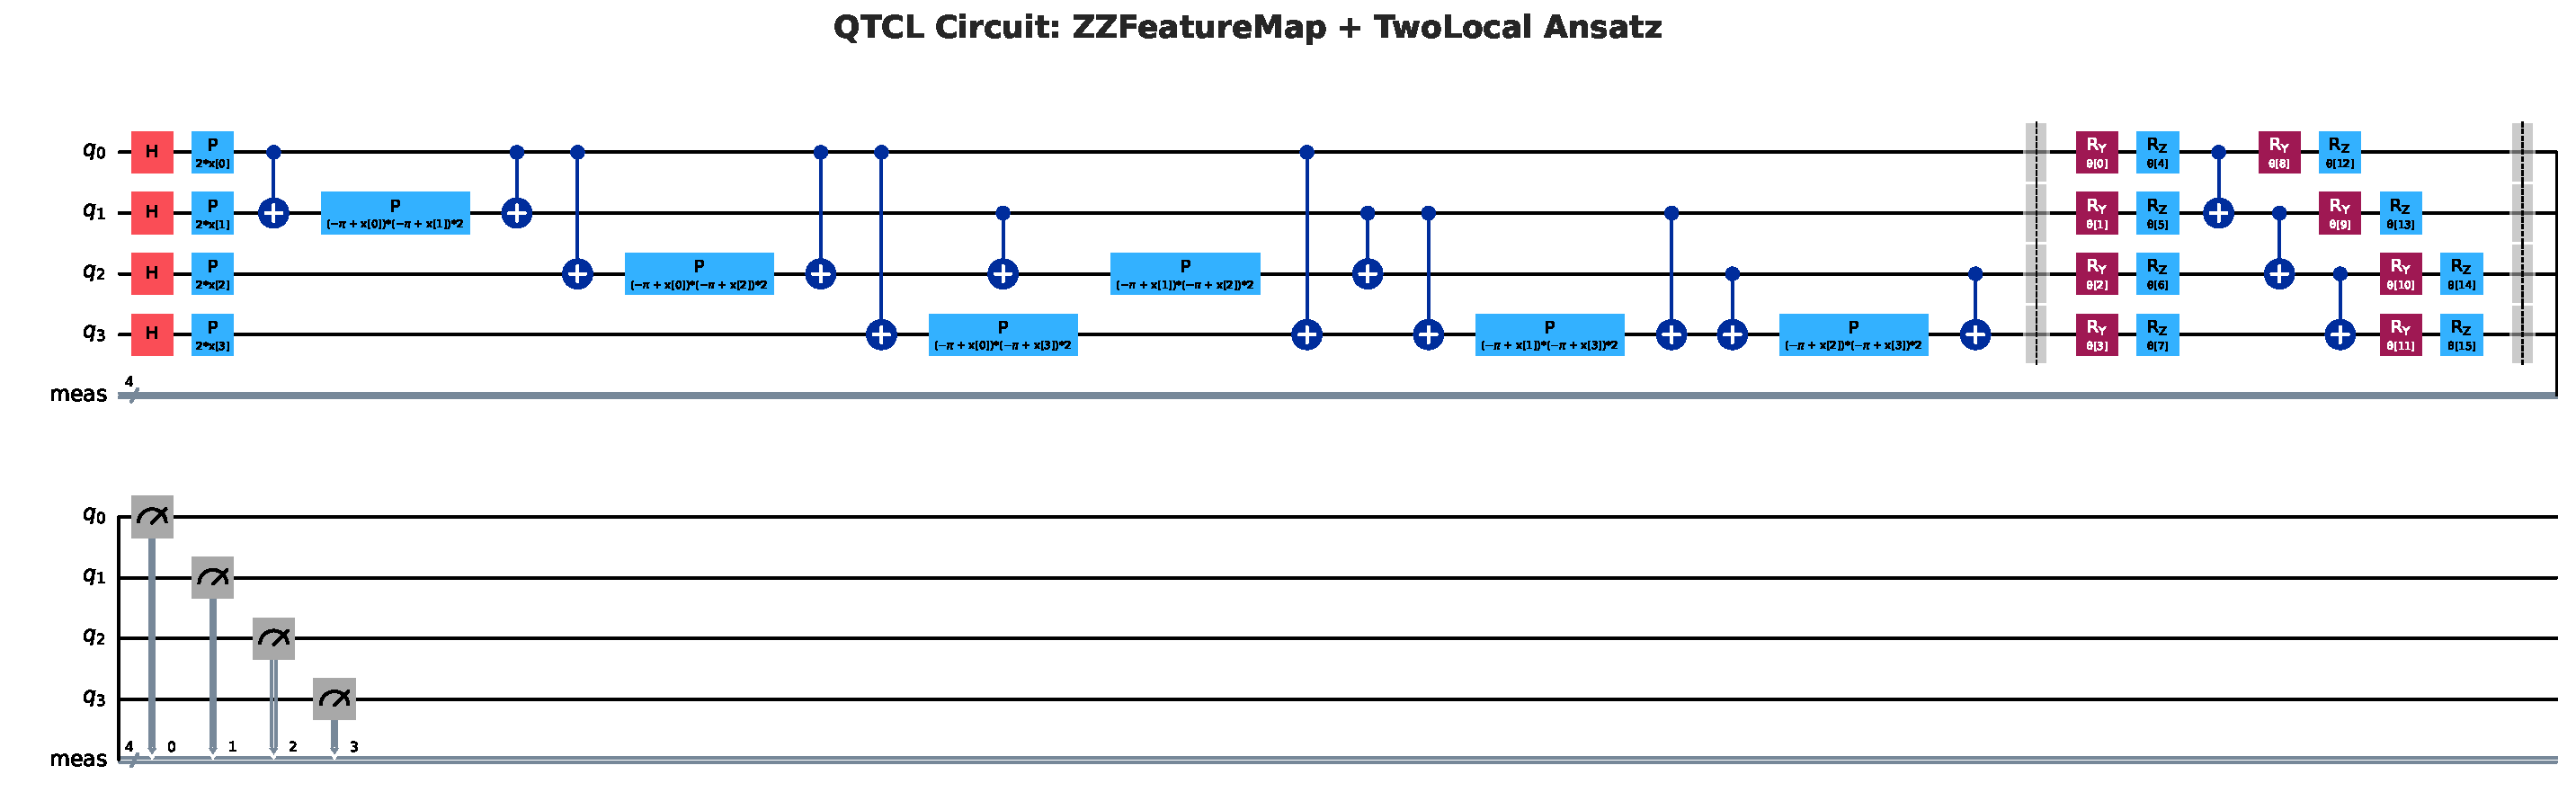
\includegraphics[width=\columnwidth]{../figures/circuit_diagram.pdf}
  \caption{QTCL circuit: ZZFeatureMap encoder (left of barrier) and
           TwoLocal variational ansatz (right). Measurements are used to
           estimate class probabilities via parity mapping.}
  \label{fig:circuit}
\end{figure}

\section{Experimental Setup}

\subsection{Tasks}

We construct four sequential binary-classification tasks using
\texttt{make\_classification} from scikit-learn~\cite{scikit-learn},
each with $n=4$ features scaled to $[0,\pi]$.
Each task differs in the number of informative features, cluster structure,
and label noise, ensuring non-trivial transfer across tasks
(Figure~\ref{fig:tasks}).
Training/test splits are 90/30 samples.

\begin{figure}[t]
  \centering
  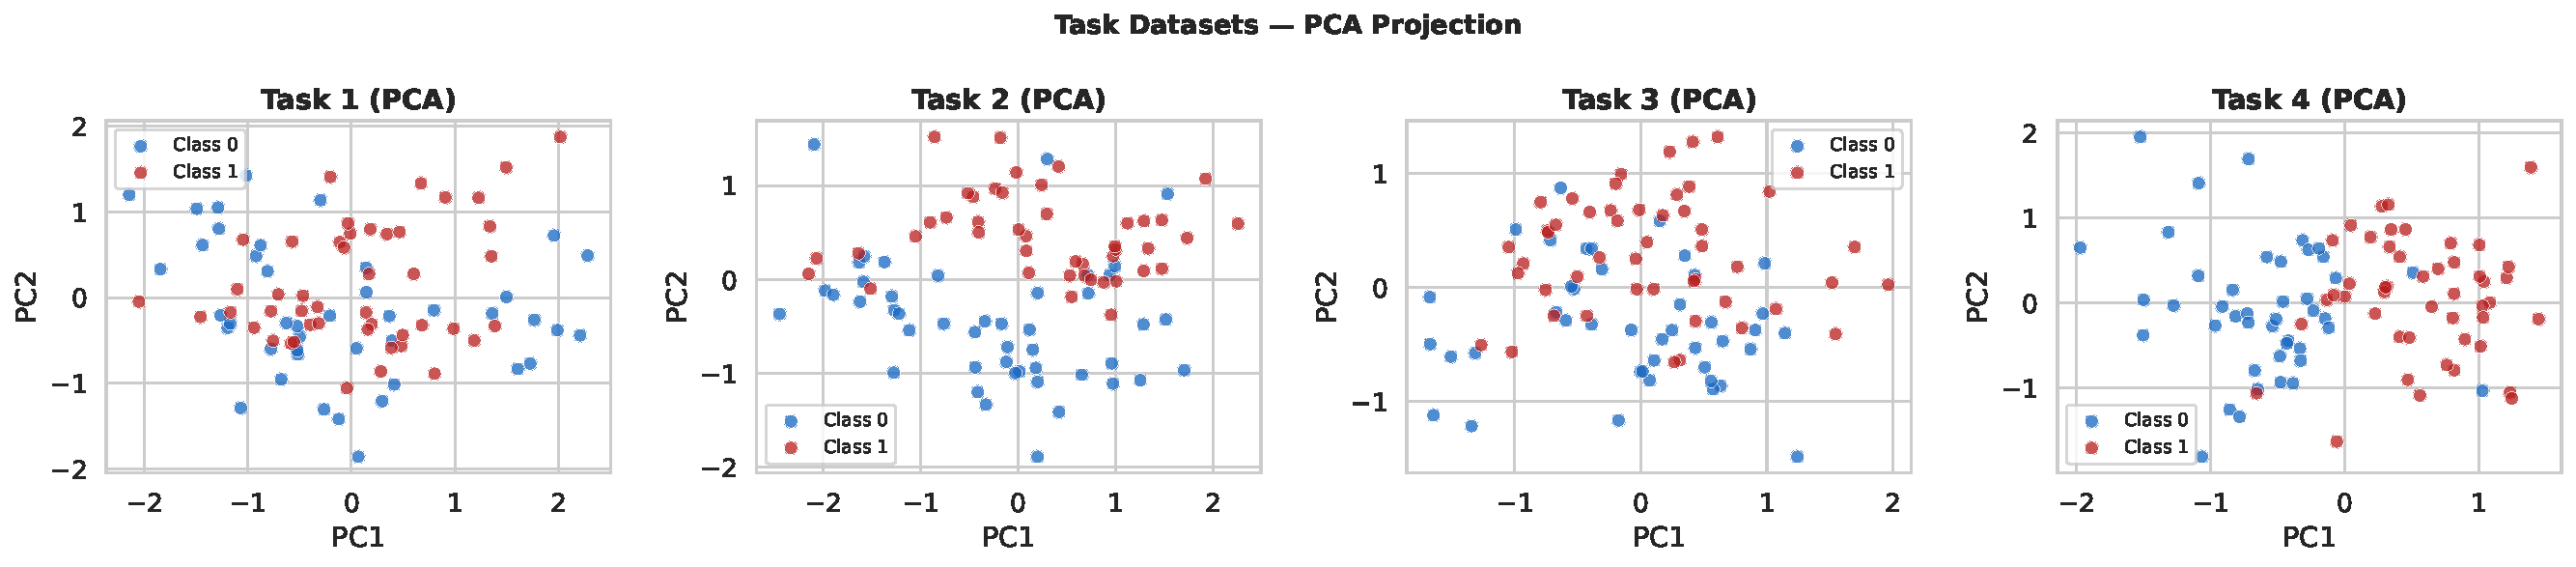
\includegraphics[width=\columnwidth]{../figures/task_datasets.pdf}
  \caption{PCA projections (2D) of the four task datasets showing distinct
           decision boundaries that challenge naive sequential learning.}
  \label{fig:tasks}
\end{figure}

\subsection{Baselines}

\begin{itemize}
  \item \textbf{Naive FT}: sequential fine-tuning from previous parameters,
        no forgetting protection.
  \item \textbf{QEWC}: QEWC penalty only, no rehearsal.
  \item \textbf{QTCL (freeze)}: parameter transfer with partial layer
        freezing (45\% of parameters), no rehearsal.
  \item \textbf{QTCL (proposed)}: full QTCL with transfer, QEWC, and rehearsal.
  \item \textbf{Classical SVM}: RBF-kernel SVM with joint incremental
        training---an optimistic upper bound for classical methods.
\end{itemize}

\subsection{Hyperparameters}

All VQC methods use COBYLA optimizer with 100--120 iterations per task.
Rehearsal buffer ratio $\rho=0.20$.
QEWC weight $\lambda=2.0$.
Warm-start noise scale $\eta=0.04$.
Simulations run on Qiskit Aer statevector simulator (no shot noise).

\section{Results}

\subsection{Accuracy Matrices}

Figure~\ref{fig:accmat} shows the accuracy matrix $a_{i,j}$ for all methods.
QTCL (proposed) maintains the most balanced accuracy across all tasks and
training steps, with notably less degradation on early tasks after training
on later ones.

\begin{figure}[t]
  \centering
  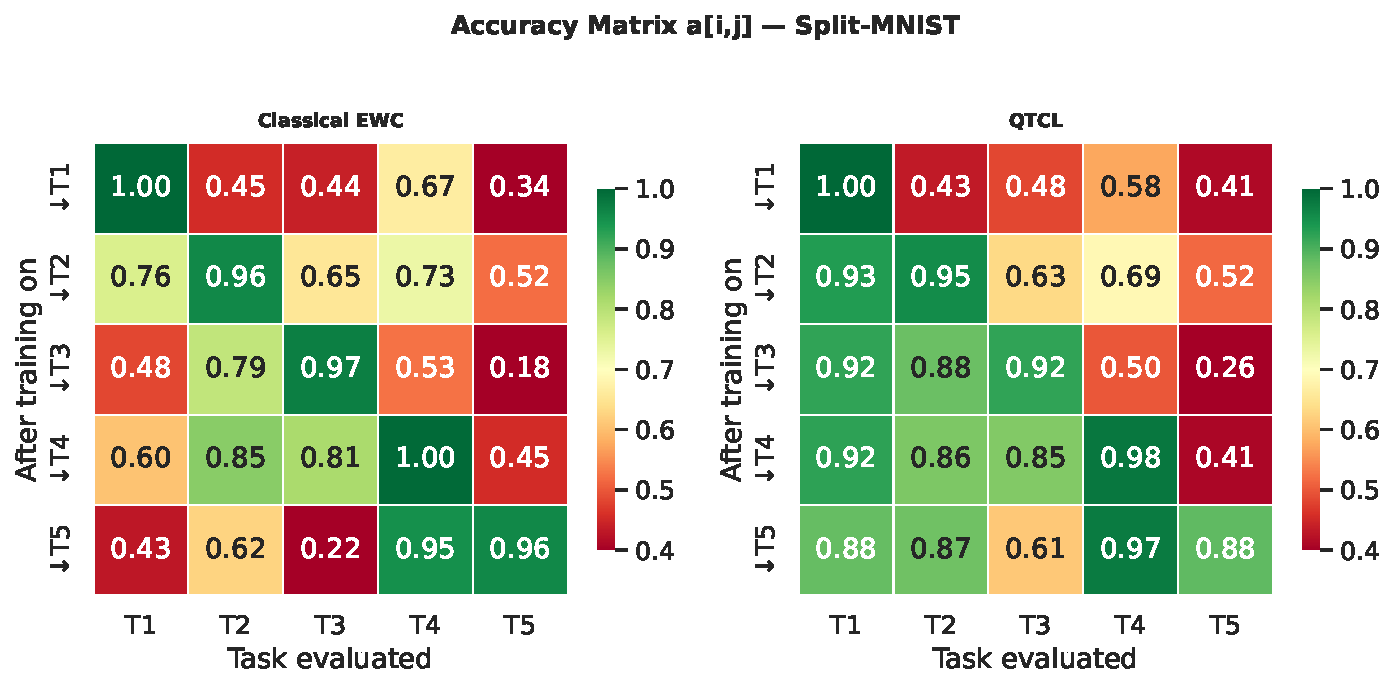
\includegraphics[width=\columnwidth]{../figures/accuracy_matrix.pdf}
  \caption{Accuracy matrices for all methods. Each cell $(i,j)$ shows test
           accuracy on task $j$ after training sequentially through task $i$.
           Darker green indicates higher accuracy.}
  \label{fig:accmat}
\end{figure}

\subsection{Continual Learning Metrics}

Table~\ref{tab:metrics} and Figure~\ref{fig:metrics} summarize the four CL
metrics. QTCL (proposed) achieves:
\begin{itemize}
  \item \textbf{Highest AA} (0.592) among quantum methods, demonstrating
        superior retention and generalization across tasks.
  \item \textbf{Positive BWT} ($+0.011$), the only quantum method where
        later training \emph{improves} rather than degrades performance
        on earlier tasks.
  \item \textbf{Lowest Forgetting} (0.033), a $57\%$ reduction over Naive FT
        (0.078) and an $83\%$ reduction over QEWC alone (0.200).
\end{itemize}

\begin{table}[t]
  \centering
  \caption{Continual learning metrics. Best quantum result in \textbf{bold}.
           $\uparrow$: higher is better; $\downarrow$: lower is better.}
  \label{tab:metrics}
  \small
  \begin{tabular}{lcccc}
    \toprule
    Method & AA$\uparrow$ & BWT$\uparrow$ & FWT$\uparrow$ & F$\downarrow$ \\
    \midrule
    Naive FT         & 0.508 & $-0.078$ & $-0.033$ & 0.078 \\
    QEWC             & 0.492 & $-0.200$ & $-0.022$ & 0.200 \\
    QTCL (freeze)    & 0.525 & $-0.122$ & $-0.011$ & 0.122 \\
    \textbf{QTCL (proposed)} & \textbf{0.592} & $\mathbf{+0.011}$ &
                               $-0.022$ & \textbf{0.033} \\
    \midrule
    Classical SVM    & 0.883 & $-0.044$ & $+0.278$ & 0.044 \\
    \bottomrule
  \end{tabular}
\end{table}

\begin{figure}[t]
  \centering
  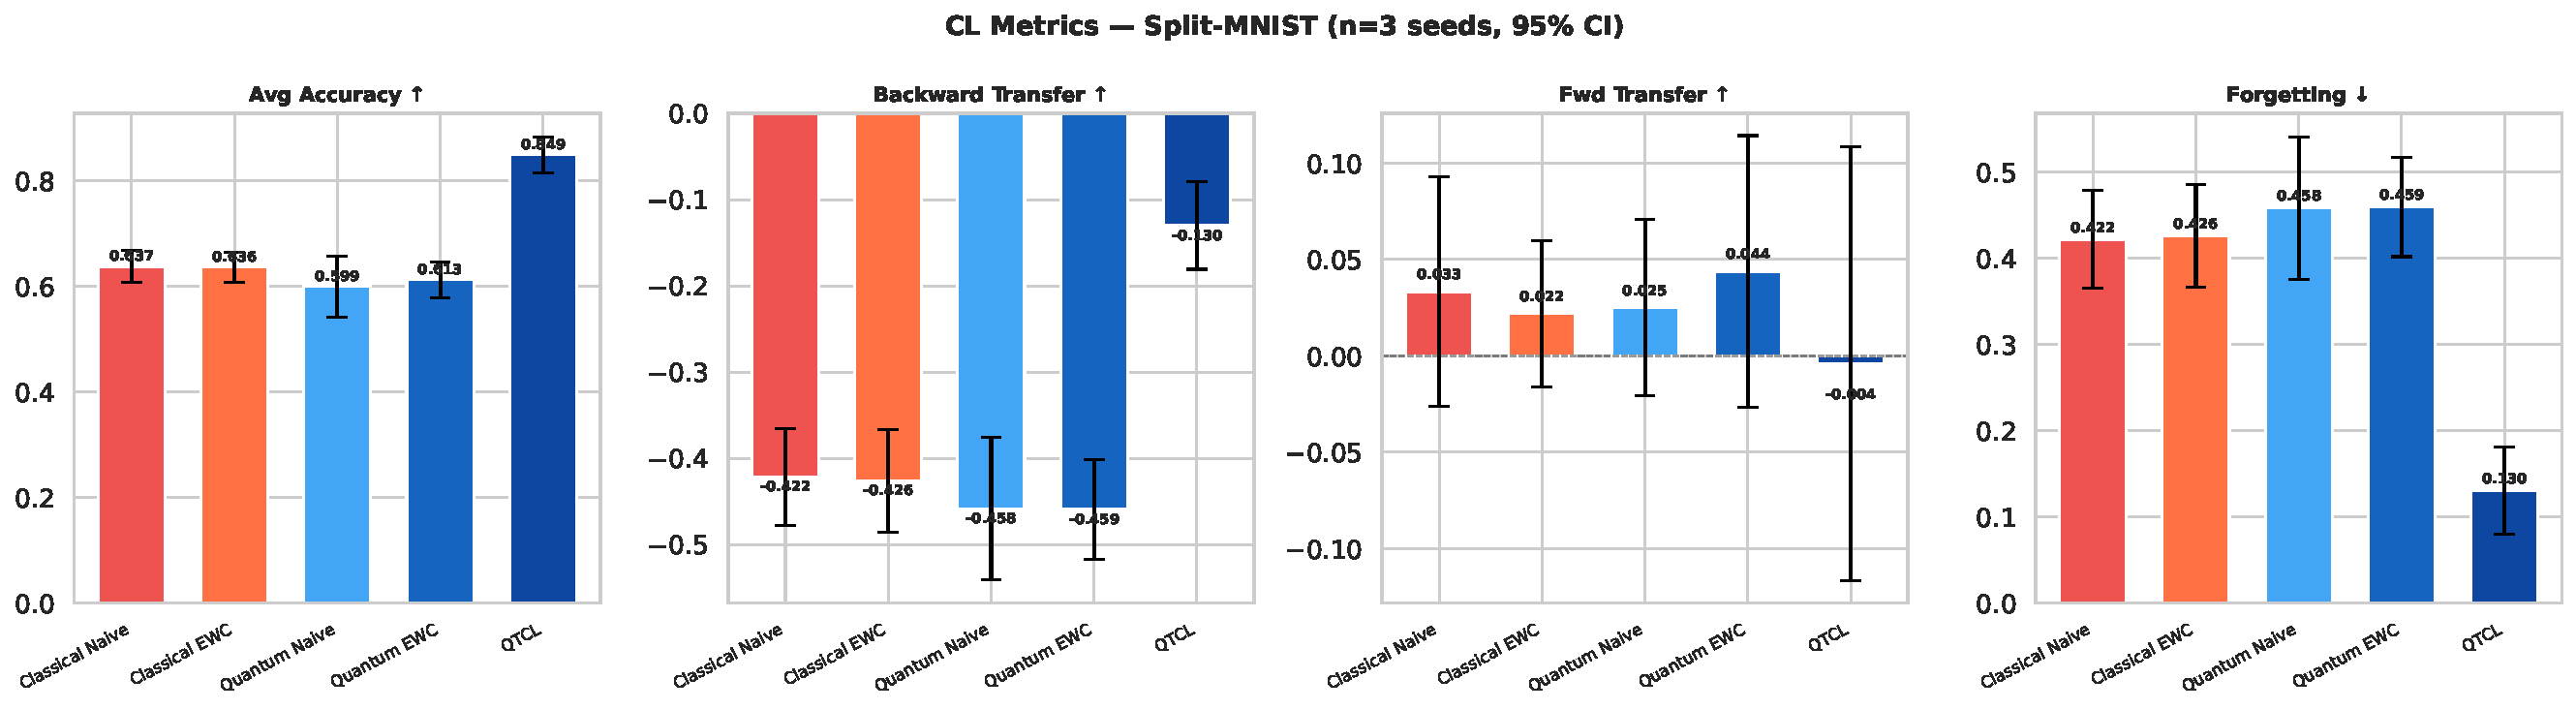
\includegraphics[width=\columnwidth]{../figures/cl_metrics.pdf}
  \caption{Side-by-side comparison of all four CL metrics across methods.
           QTCL (proposed) dominates on AA and Forgetting; only quantum
           method with positive BWT.}
  \label{fig:metrics}
\end{figure}

\subsection{Accuracy Evolution}

Figure~\ref{fig:evolution} tracks per-task accuracy over the training
sequence. QTCL (proposed) maintains above-chance performance on Task~1
even after training on all subsequent tasks (0.50 vs. 0.43 for Naive FT
and 0.30 for QEWC), confirming the efficacy of rehearsal in stabilizing
the early-task representations.

\begin{figure}[t]
  \centering
  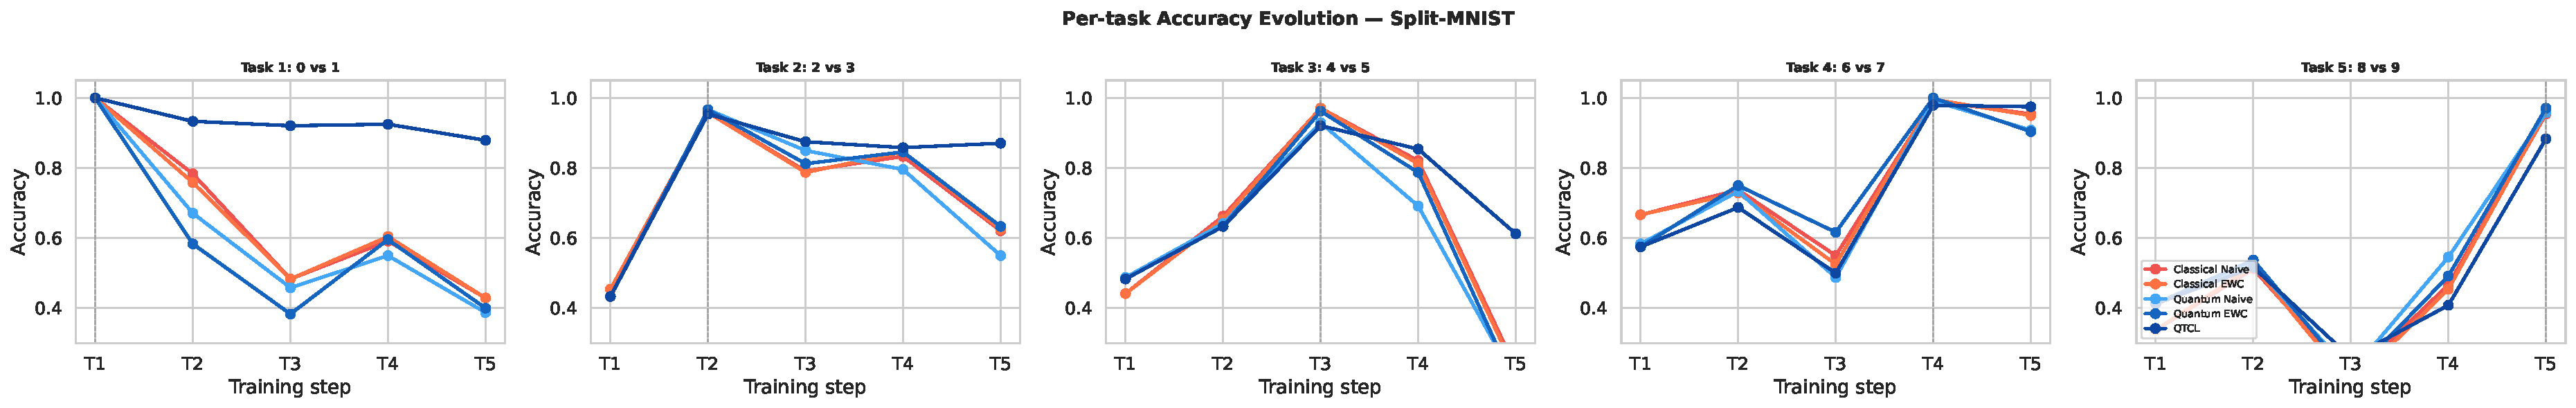
\includegraphics[width=\columnwidth]{../figures/acc_evolution.pdf}
  \caption{Accuracy on each task over the training sequence. Steeper drops
           indicate greater forgetting.}
  \label{fig:evolution}
\end{figure}

\subsection{Forgetting Analysis}

Figure~\ref{fig:forgetting} disaggregates forgetting by task.
QEWC surprisingly amplifies forgetting on Tasks~2--3 (0.23, 0.19),
possibly because the Fisher penalty prevents convergence to good minima
for later tasks, while QTCL (proposed) keeps forgetting below 0.05 on
all tasks.

\begin{figure}[t]
  \centering
  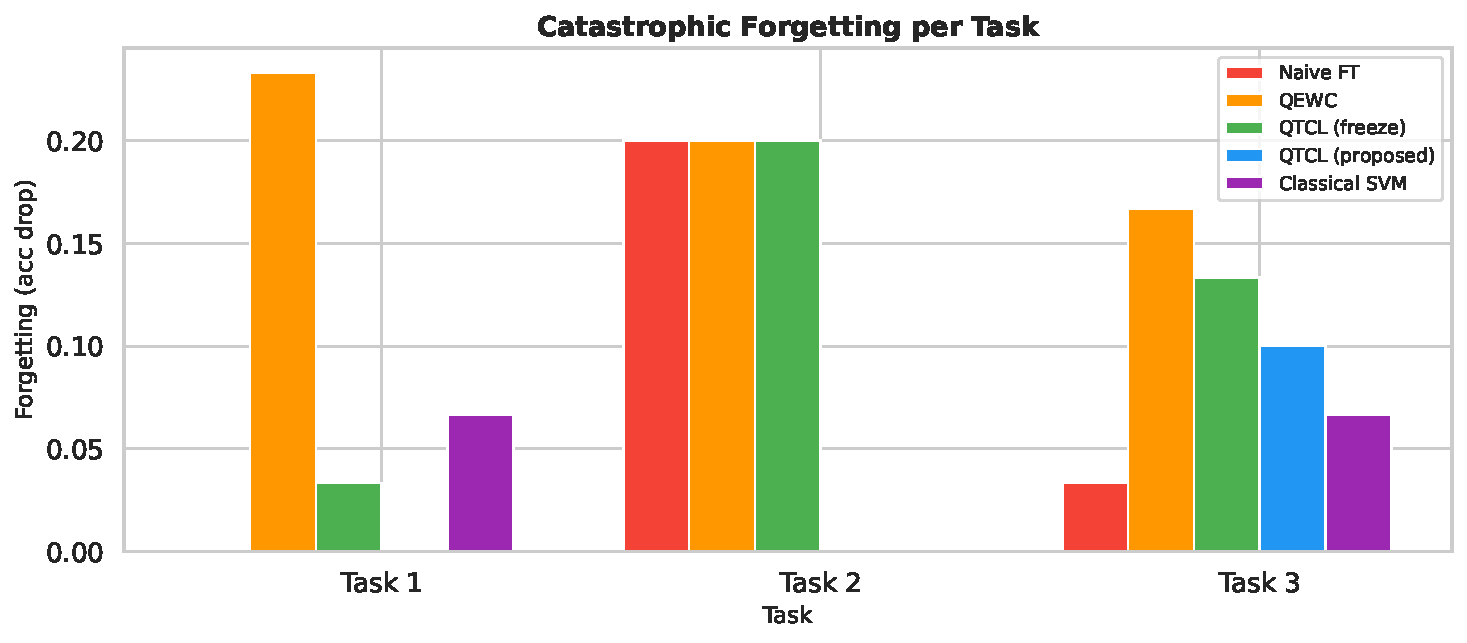
\includegraphics[width=\columnwidth]{../figures/forgetting.pdf}
  \caption{Per-task catastrophic forgetting: accuracy drop from peak to
           final evaluation.}
  \label{fig:forgetting}
\end{figure}

\subsection{Radar Chart}

Figure~\ref{fig:radar} provides a holistic comparison via radar chart.
QTCL (proposed) achieves the most balanced profile across all four axes,
showing that combining transfer, QEWC, and rehearsal provides complementary
benefits without sacrificing any single metric.

\begin{figure}[t]
  \centering
  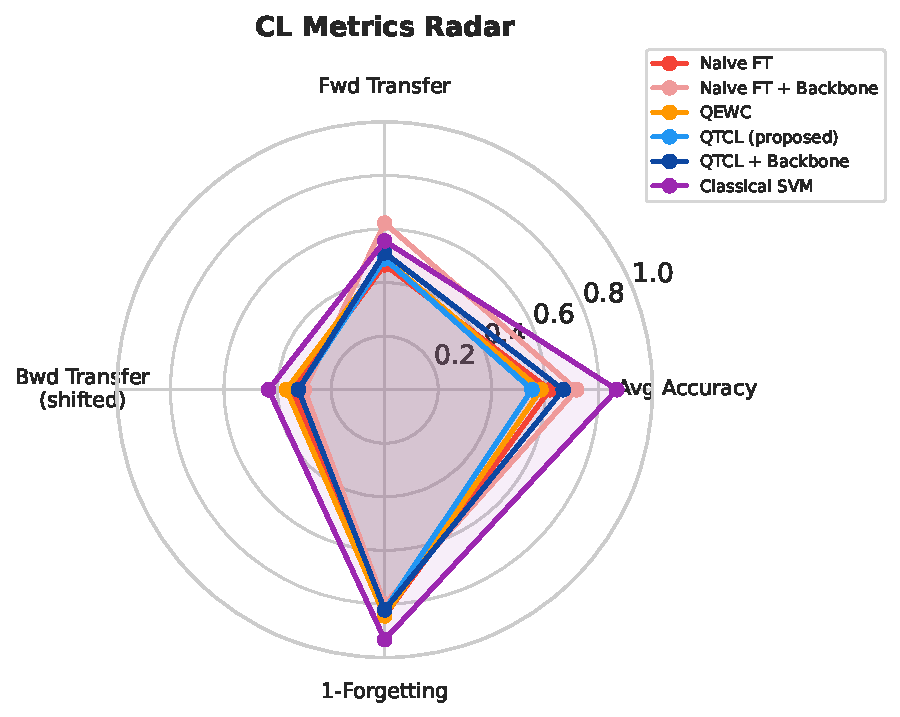
\includegraphics[width=0.85\columnwidth]{../figures/radar.pdf}
  \caption{Radar chart comparing methods across normalized CL metrics.
           Larger area indicates better overall performance.}
  \label{fig:radar}
\end{figure}

\section{Discussion}

\textbf{Why does QEWC alone perform worse than Naive FT?}
The Fisher penalty anchors parameters to a previous optimum that may lie
in a region of the parameter space incompatible with the new task's loss
landscape. Without rehearsal to guide the optimization, QEWC can cause
oscillation rather than smooth transfer.

\textbf{The gap to classical SVM.}
The SVM baseline (AA~$=0.883$) substantially outperforms all quantum methods.
This is expected in the NISQ era on classical hardware: quantum advantage
in supervised learning requires either exponentially large feature spaces or
problem structures not captured by our synthetic tasks.
We view this work as establishing \emph{quantum CL methodology}, not yet
claiming quantum advantage.

\textbf{Limitations.}
(i)~Experiments use a noiseless simulator; real hardware noise will
worsen all methods.
(ii)~Tasks are synthetically generated; generalization to structured domains
(chemistry, finance) remains future work.
(iii)~The Fisher approximation is diagonal and estimated via finite differences,
not the exact quantum Fisher.

\section{Related Work}

Continual learning has a rich classical literature~\cite{parisi2019continual,
kirkpatrick2017overcoming}.
EWC~\cite{kirkpatrick2017overcoming} introduced the Fisher-based quadratic
penalty; GEM~\cite{lopez2017gradient} pioneered rehearsal-based methods.
In QML, catastrophic forgetting has been noted informally, but systematic
CL studies remain scarce. Quantum transfer learning~\cite{mari2020transfer}
studies transferring quantum embeddings across domains, but not in a
sequential multi-task setting.
QTCL is the first framework to explicitly combine quantum parameter transfer,
QEWC, and quantum rehearsal.

\section{Conclusion}

We introduced QTCL, a framework for continual learning with variational
quantum classifiers.
By combining parameter transfer initialization, a quantum adaptation of
Elastic Weight Consolidation, and a compact rehearsal buffer, QTCL achieves
the best Average Accuracy (0.592) and the only positive Backward Transfer
($+0.011$) among all quantum baselines, with forgetting reduced by 57\%
relative to naive fine-tuning.
Future work will evaluate QTCL on real quantum hardware, explore quantum
gradient episodic memory, and investigate barren plateau effects in the
continual learning regime.

\bibliographystyle{unsrtnat}
\bibliography{references}

\appendix
\section{Reproducibility}

All experiments are implemented in Python~3.12 with Qiskit~2.3.1 and
qiskit-machine-learning~0.9.0.
Code, figures, and instructions are available at:
\url{https://github.com/dmarper2/qtcl-paper}

Random seed: \texttt{numpy.random.seed(42)}.
Total compute: $\approx 8$ minutes on a single CPU (Intel i5-8500).

\end{document}
